% ===========================================================================
\subsection{Two-piece hexagonal cavity: full Nb$_3$Sn coating}\label{sec:2piecenb3sn}
% ===========================================================================

Cutting the cavity from eighteen interfaces to one motivated the two-piece design, built under a DOE Office of Science Graduate Student Research fellowship with Dr.\ G.\ Carosi at LLNL. The inner surface stayed hexagonal so that the electromagnetic models developed for the eight-piece cavity still applied and so that the pieces still fit the sputtering chamber. Walls thickened to a \qty{2}{\milli\meter} minimum, which removes the flexure that made the eight-piece readings sensitive to hand pressure (Fig.~\ref{fig:2piececavityCu}).

\begin{figure}[htb]
    \centering
    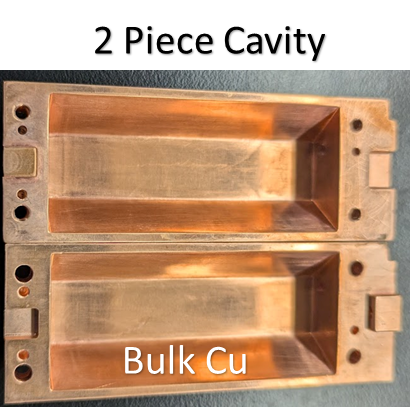
\includegraphics[width=0.7\linewidth]{images/AndreCavity/2piececavityCu.png}
    \caption{Two-piece hexagonal copper cavity.}
    \label{fig:2piececavityCu}
\end{figure}

\subsubsection{Copper baseline and the value of surface preparation}

The bare two-piece cavity was measured at each stage of surface preparation, and the result is the clearest lesson in this work (Fig.~\ref{fig:CuCavitiesRsvsT}). Hand-polished to 1200 grit it gave $Q = 12{,}000$ at room temperature and $Q = 35{,}000$ at \qty{4}{\kelvin}. Room-temperature $Q$ rose by a third over the eight-piece cavity, confirming that the single seam leaks less. Cold $Q$ did not move, which places the remaining loss in the copper surface rather than in the seam. The LLNL chemical etch then raised $Q$ to $49{,}000$, and the \qty{250}{\degreeCelsius} argon anneal raised it to $55{,}000$. Chemistry and heat treatment together bought \qty{57}{\percent}, against a simulated ceiling of $76{,}000$ for seamless RRR-300 copper at \qty{11}{\giga\hertz}.

\begin{figure}[htb]
    \centering
    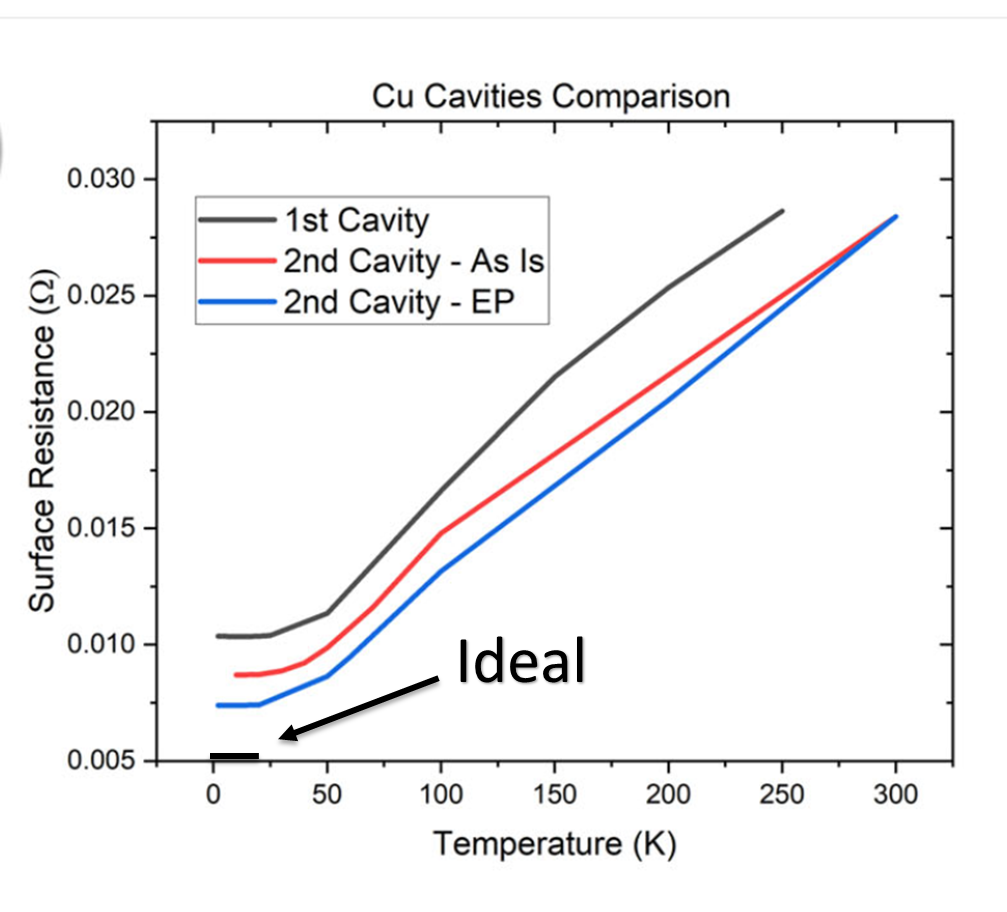
\includegraphics[width=0.7\linewidth]{images/AndreCavity/CuCavitiesRsvsT.png}
    \caption[Surface resistance versus temperature for both copper cavity designs and successive surface treatments.]{Surface resistance versus temperature for the eight-piece and two-piece copper cavities at successive stages of surface preparation. The \qty{5}{\milli\ohm} ideal line is the simulated value for the same geometry with RRR-300 copper at \qty{11}{\giga\hertz}.}
    \label{fig:CuCavitiesRsvsT}
\end{figure}

\subsubsection{Coating and measurement}

The etched and annealed cavity was coated over its full inner surface with the Nb-first recipe, using a HiPIMS Ta barrier (Fig.~\ref{fig:2piececavityrecipe}). It was measured at ASC in the PPMS from \qty{2}{\kelvin} to \qty{20}{\kelvin}, then shipped to LLNL for dilution-refrigerator measurement to \qty{50}{\milli\kelvin} (Fig.~\ref{fig:LLNLDilutionQtest}).

\begin{figure}[htb]
    \centering
    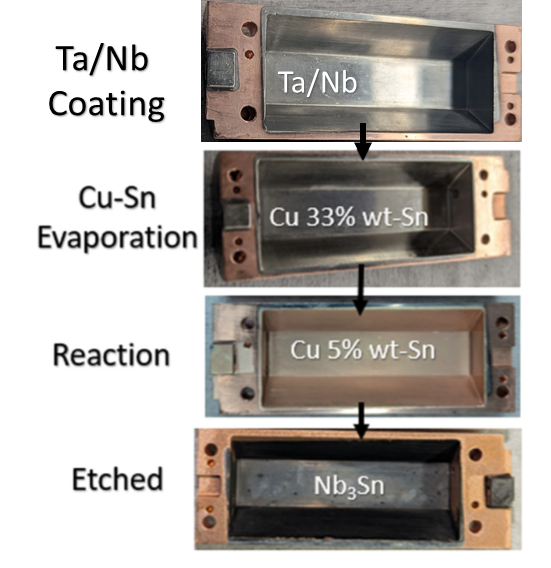
\includegraphics[width=0.7\linewidth]{images/AndreCavity/2piececavityrecipe.png}
    \caption{Down-selected Nb-first recipe as applied to the two-piece cavity.}
    \label{fig:2piececavityrecipe}
\end{figure}

\begin{figure}[htb]
    \centering
    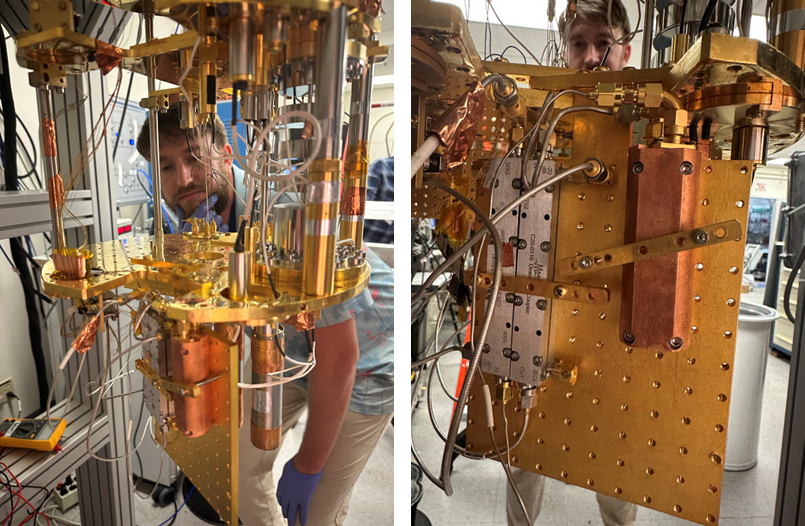
\includegraphics[width=0.85\linewidth]{images/AndreCavity/LLNLDilutionQtest.png}
    \caption{Dilution refrigerator setup at LLNL for millikelvin $Q$ measurements of the two-piece cavity.}
    \label{fig:LLNLDilutionQtest}
\end{figure}

The loaded quality factor held constant at $Q_L = 77{,}000$ ($R_s = \qty{5}{\milli\ohm}$) from \qty{50}{\milli\kelvin} to \qty{300}{\milli\kelvin}, and measured $Q_L = 59{,}000$ ($R_s = \qty{6}{\milli\ohm}$) at \qty{2}{\kelvin} (Fig.~\ref{fig:2pieceCavityResults}). Applying the \qty{10}{\percent} weak-coupling correction gives $Q_0 \approx 85{,}000$ at \qty{50}{\milli\kelvin} and $Q_0 \approx 65{,}000$ at \qty{2}{\kelvin}. A flat $Q$ across a factor of six in temperature confirms that $R_\text{BCS}$ is negligible below \qty{300}{\milli\kelvin} and that what remains is residual resistance.

\begin{figure}[htb]
    \centering
    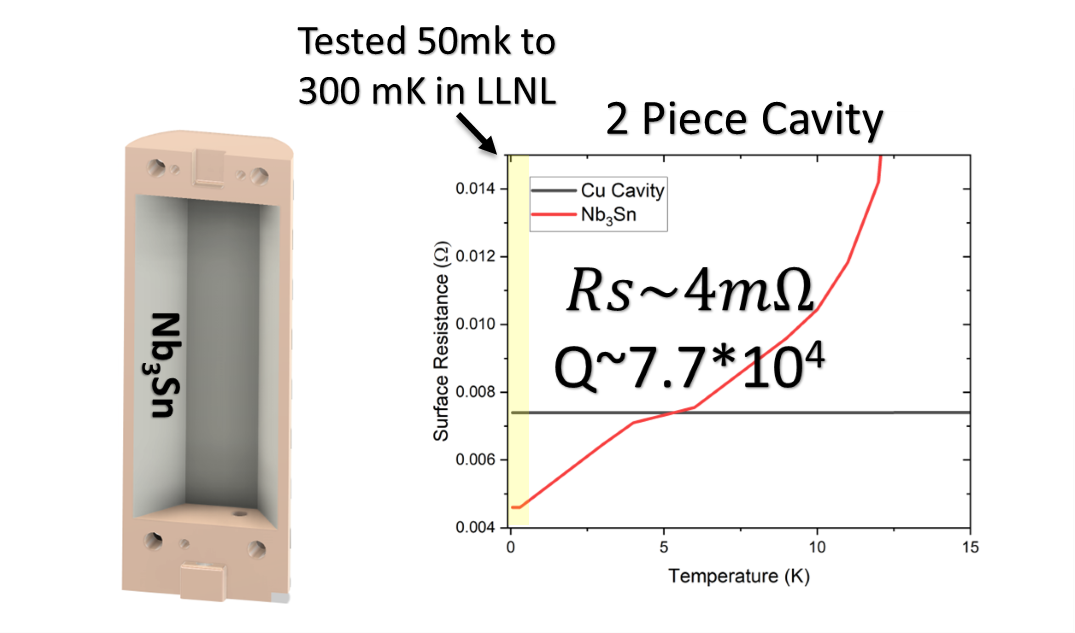
\includegraphics[width=0.85\linewidth]{images/AndreCavity/2pieceCavityResults.png}
    \caption{Model and surface resistance versus temperature for the two-piece Nb$_3$Sn-coated cavity.}
    \label{fig:2pieceCavityResults}
\end{figure}

\subsubsection{Corrections for uncoated endcaps and seam leakage}

Inspection after measurement found that the film had peeled from both endcaps during the APS etch (Fig.~\ref{fig:EdgeEffect2piece}). Line-of-sight deposition had not adhered to surfaces perpendicular to the flux. The walls also carried dark spots, scratches, and rough patches from surface preparation and from deposition onto steeply inclined faces. Roughly one third of the resonating surface was therefore bare copper, and the measured $Q_L = 77{,}000$ mixes two materials and one leaking seam.

\begin{figure}[htb]
    \centering
    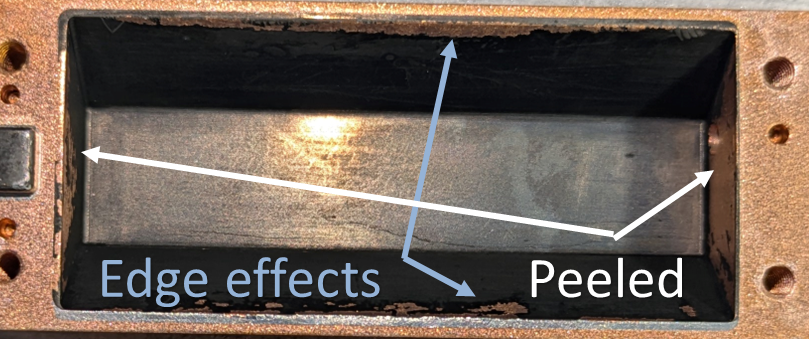
\includegraphics[width=0.75\linewidth]{images/AndreCavity/EdgeEffect2piece.png}
    \caption{Coating defects at the endcaps and edge regions of the two-piece cavity, showing delamination and non-uniform coverage.}
    \label{fig:EdgeEffect2piece}
\end{figure}

Two corrections separate the Nb$_3$Sn contribution, following Appendix~\ref{app:Qcorrection}. For a hybrid cavity with $G_\text{total} = \qty{350}{\ohm}$ split as $G_\text{Cu} = \qty{1050}{\ohm}$ over one third of the surface and $G_{\text{Nb}_3\text{Sn}} = \qty{525}{\ohm}$ over two thirds,

\begin{equation}
    \frac{1}{Q_\text{meas}} = \frac{R_{s,\text{Cu}}}{G_\text{Cu}} + \frac{R_{s,\text{Nb}_3\text{Sn}}}{G_{\text{Nb}_3\text{Sn}}} .
\end{equation}

Inserting the measured copper value $R_{s,\text{Cu}} = \qty{6.36}{\milli\ohm}$ at \qty{50}{\milli\kelvin} gives $R_{s,\text{Nb}_3\text{Sn}} = \qty{3.64}{\milli\ohm}$, so a fully coated cavity would reach

\begin{equation}
    Q_{\text{Nb}_3\text{Sn,full}} = \frac{G_\text{total}}{R_{s,\text{Nb}_3\text{Sn}}} = \frac{\qty{350}{\ohm}}{\qty{3.64}{\milli\ohm}} = 9.6\times10^{4} .
\end{equation}

The seam correction uses copper as its own reference. The measured copper cavity reached $55{,}000$ against a simulated seamless $76{,}000$, so

\begin{equation}
    \alpha = \frac{Q_\text{Cu,ideal}}{Q_\text{Cu,meas}} = \frac{76{,}000}{55{,}000} = 1.38 ,
\end{equation}

and assuming the same fractional leakage for both materials,

\begin{equation}
    Q_{\text{Nb}_3\text{Sn,corrected}} = 1.38 \times 9.6\times10^{4} = 1.3\times10^{5} .
\end{equation}

With the weak-coupling correction this is $Q_0 \approx 1.4\times10^{5}$ at \qty{50}{\milli\kelvin} and zero field, a factor of \num{2.5} above the bare copper reference. The number rests on assumptions listed in Appendix~\ref{app:Qcorrection}, chiefly that the coated fraction is one third and that seam leakage is material-independent.
